\documentclass[journal,conference]{IEEEtran}


% correct bad hyphenation here
\hyphenation{op-tical net-works semi-conduc-tor}
\usepackage{amsmath}
\usepackage{comment}
%\usepackage{cases}
%\usepackage{subeqnarray}
\usepackage{booktabs}
\usepackage{subfigure}
\usepackage{xcolor}
\usepackage{listings}
\lstset{
  basicstyle=\fontsize{9}{10}\selectfont\ttfamily,
  numbers=left,
  numberstyle= \tiny,
  keywordstyle= \color{ blue!70},
  commentstyle= \color{red!50!green!50!blue!50},
  frame=single,
  rulesepcolor= \color{ red!20!green!20!blue!20} ,
  escapeinside=``,
  xleftmargin=1.5em,xrightmargin=0em, aboveskip=1em,
  framexleftmargin=2em,
  showstringspaces=false,
  showtabs=false,
  breaklines=true
}
\lstdefinelanguage{Solidity}
{
  morekeywords={contract, mapping, address, uint, private, function, public, if, payable},
  morecomment=[l]{//},
  morestring=[b]"
}


\usepackage{multicol}
\usepackage{lipsum}
\usepackage{mathtools}
\usepackage{cuted}

\usepackage{amsmath}
\usepackage{extpfeil}
\usepackage{mathpartir}
\usepackage[mathscr]{eucal}

\usepackage{hyperref}
\usepackage{cleveref}

% \usepackage{fontspec}

% \usepackage{CJK}

\crefformat{section}{\S#2#1#3} % see manual of cleveref, section 8.2.1
\crefformat{subsection}{\S#2#1#3}
\crefformat{subsubsection}{\S#2#1#3}

\begin{document}

% \newfontfamily\cl{Consolas}
% \newcommand{\code}[1]{{\cl #1}}
\newcommand{\code}[1]{\colorbox[rgb]{0.95,0.95,0.95}{#1}}
% \newcommand{\code}[1]{#1}

%
% paper title
% Titles are generally capitalized except for words such as a, an, and, as,
% at, but, by, for, in, nor, of, on, or, the, to and up, which are usually
% not capitalized unless they are the first or last word of the title.
% Linebreaks \\ can be used within to get better formatting as desired.
% Do not put math or special symbols in the title.
\title{Improve SSD with Feature Fusion, \\IOU Loss and Super Resolution}
%
%
% author names and IEEE memberships
% note positions of commas and nonbreaking spaces ( ~ ) LaTeX will not break
% a structure at a ~ so this keeps an author's name from being broken across
% two lines.
% use \thanks{} to gain access to the first footnote area
% a separate \thanks must be used for each paragraph as LaTeX2e's \thanks
% was not built to handle multiple paragraphs
%

\author{
  Jingyu~Li,~\IEEEmembership{SJTU,}
  Haoping~Chen,~\IEEEmembership{SJTU,}
  Huangfei~Jiang,~\IEEEmembership{SJTU,}
}

% The paper headers
\markboth{Journal of \LaTeX\ Class Files,~Vol.~13, No.~9, September~2014}%
{Shell \MakeLowercase{\textit{et al.}}: Bare Demo of IEEEtran.cls for Journals}
% The only time the second header will appear is for the odd numbered pages
% after the title page when using the twoside option.
%
% *** Note that you probably will NOT want to include the author's ***
% *** name in the headers of peer review papers.                   ***
% You can use \ifCLASSOPTIONpeerreview for conditional compilation here if
% you desire.


% make the title area
\maketitle

% As a general rule, do not put math, special symbols or citations
% in the abstract or keywords.
\begin{abstract}
  In this project
\end{abstract}

% Note that keywords are not normally used for peerreview papers.
\begin{IEEEkeywords}
  OBI recognition, CNN, template matching, data augmentation.
\end{IEEEkeywords}


\IEEEpeerreviewmaketitle



\section{Introduction}
\IEEEPARstart{O}{racle}


% ljy
\section{SSD Baseline}
Single Shot Multibox Detector (SSD) is an end-to-end convolutional neural network for object detection. The original paper \cite{ssd} demonstrates two variants of the model called the SSD300 and the SSD512. The suffixes represent the size of the input image. They have the same principles, although their structures have a slight difference.

As a baseline model, we choose SSD300 and reimplement it in PyTorch. The top functions of SSD network structure are shown in \code{ssd.py}. This section will focus on the structure of SSD network. The training and evaluation will be discussed in the experiment section.

% Unlike earlier architectures for object detection, e.g. RCNN, which consist of two distinct stages, a region proposal network that performs object localization and a classifier for detecting the types of objects in the proposed regions. However, they can be very computational expensive and therefore incapable of real-world, real-time applications. Single-shot models encapsulate both localization and detection tasks in a single network, resulting in significantly faster detections while deployable on lighter hardware.

\subsection{Network Structure Overview}
The whole SSD network can be organized into three parts

\subsubsection{Base convolutions}
It is derived from an existing image classification architecture that will provide lower-level feature maps.

SSD uses a modified VGG-16 as the base network. The first five blocks are a repetition of convolution, convolution and max pooling. Different from the original VGG-16, the remaining fully-connected layers (fc) are modified. FC8 is removed, and FC6 and FC7 are turned into convolutional layers. The base network will generate two feature maps: \code{conv4\_3} of size $38$ and \code{conv7} of size $19$ for later detection.

\subsubsection{Auxiliary convolutions}
They are added on top of the base network that will provide higher-level feature maps. SSD300 adds four extra convolution blocks to generate four more high-level feature maps \code{conv8\_2}, \code{conv9\_2}, \code{conv10\_2}, \code{conv11\_2} of size $10$, $5$, $3$, $1$.

\subsubsection{Prediction convolutions} layers that that will locate and identify objects in these feature maps, which will be discussed in more detail in the following.


All of these three structures are constructed in the function \code{multibox()}, and are named \code{vgg}, \code{extra\_layers} and \code{head}.

\subsection{Prior boxes}
The bounding box for a single object can be infinitely many. So to tackle with infinity, SSD create a finite set of bounding box configurations so that there are only thousands of precalculated and fixed potential box, known as priors.

Priors are manually but carefully chosen based on the shapes and sizes of ground truth objects in the dataset. By placing these priors at every possible location in a feature map, we also account for variety in position

In defining the priors
\begin{itemize}
  % \setlength{\itemsep}{0pt}
  % \setlength{\parsep}{0pt}
  % \setlength{\parskip}{0pt}
  \item Every prior has a scale $s$. The largest feature map \code{conv4\_3} will have priors with a scale of $0.1$, i.e. $10\%$ of image's dimensions, while the rest have priors with scales linearly increasing from $0.2$ to $0.9$. So larger feature maps have priors with smaller scales and are therefore ideal for detecting smaller objects.
  \item At each position on a feature map, there will be priors of various aspect ratios. All feature maps will have priors with ratios \code{1:1}, \code{2:1} and \code{1:2}. Later feature maps also have ratios \code{3:1}, \code{1:3} and \code{1:1}, as shown in Figure~\ref{fig:prior}.
\end{itemize}

\begin{figure}[htbp]
  \centering
  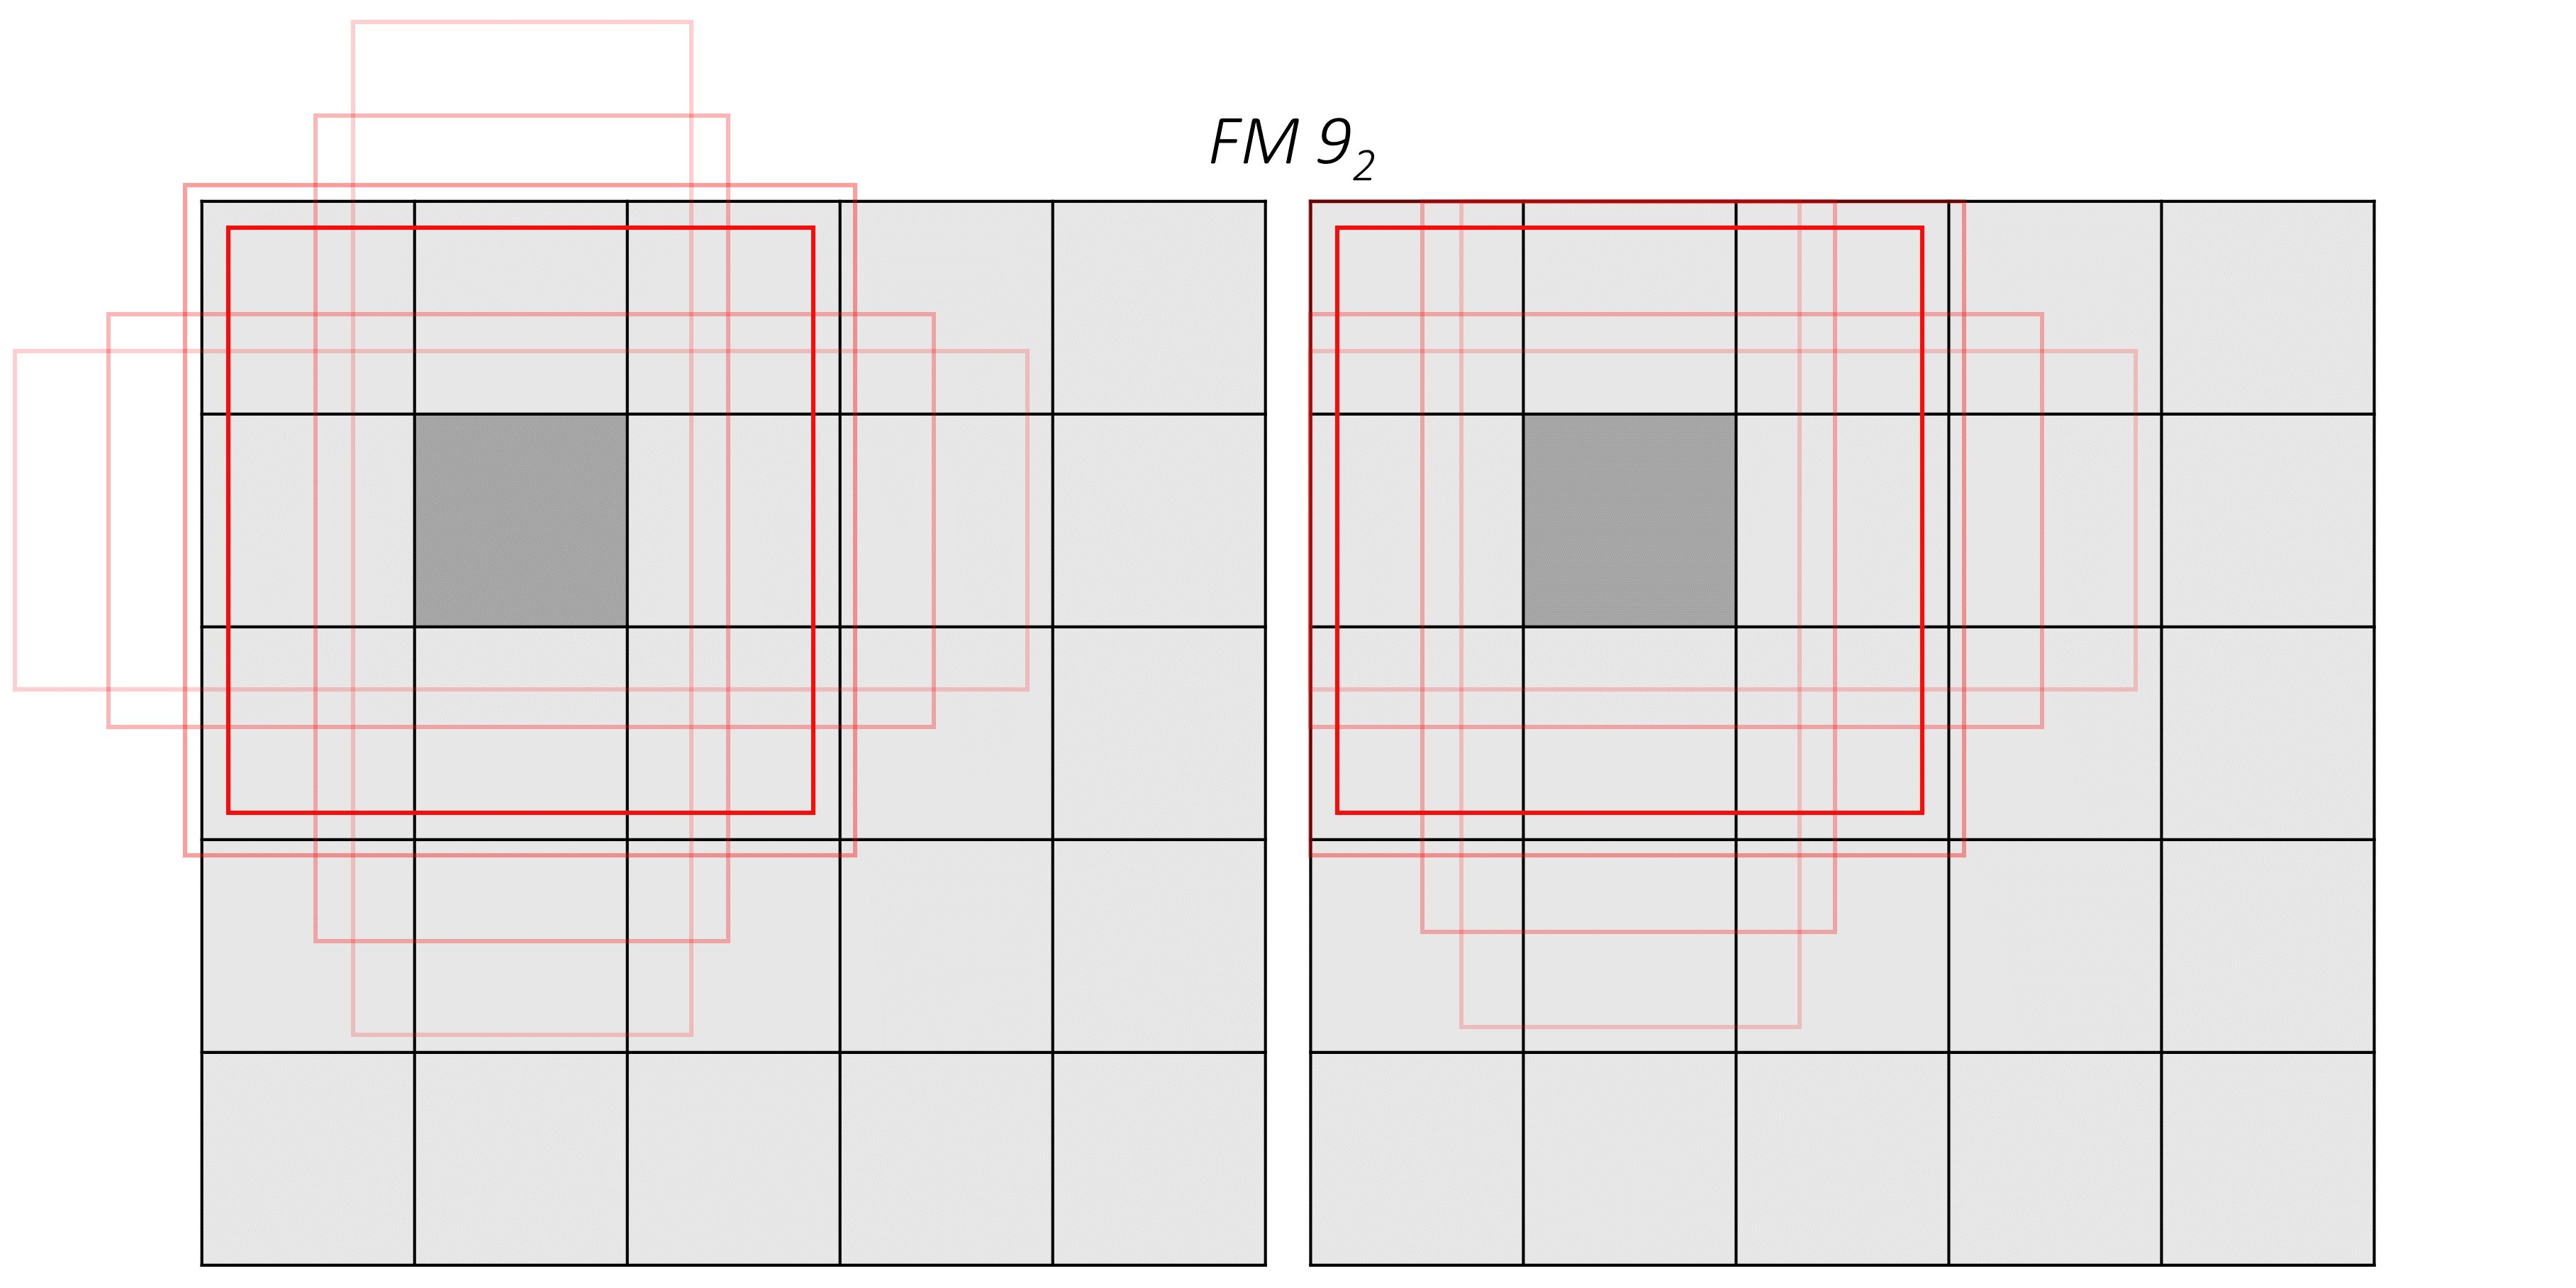
\includegraphics[width=\linewidth]{fig/priors2.jpg}
  \caption{Prior boxes for feature map 9\_2. When priors at a location overshoot the edges of the feature map, they are clipped.}\label{fig:prior}
\end{figure}

\subsection{Prediction convolutions}
We use each prior as an approximate starting point and then find out how much it needs to be adjusted to obtain a more exact prediction for a bounding box. So we need to predict the offset of the box to the priors. Besides, we also need $n$ scores for each bounding box to show its confidence in each class.

To do this in the simples manner, we use two convolutional layers for each feature map:
\begin{itemize}
  \item a localization prediction convolutional layer with a $3\times 3$ kernel evaluating at each location (i.e. with padding and stride of 1) with 4 filters for each prior present at the location, which calculate the four encoded offsets $(g_{c_x}, g_{c_y}, g_w, g_h)$ for the bounding box predicted from that prior.

  \item a class prediction convolutional layer with a $3\times 3$ kernel evaluating at each location  with $n$ filters for each prior present at the location
\end{itemize}

\subsection{Non-Maximum Suppression}
Following the above procedures, we have $8732$ candidate boxes. To eliminate the inaccurate ones, we need to use what is called Non-maximum suppression (NMS). Algorithmically, it is carried out as follows:

Upon selecting candidades for each non-background class,
\begin{enumerate}
  \item Arrange candidates for this class in order of decreasing likelihood.

  \item Consider the candidate with the highest score. Eliminate all candidates with lesser scores that have a overlap of more than, say, 0.5 with this candidate.

  \item Consider the next highest-scoring candidate still remaining in the pool. Eliminate all candidates with lesser scores that have a overlap of more than 0.5 with this candidate.

  \item Repeat until you run through the entire sequence of candidates.
\end{enumerate}

% The end result is that you will have just a single box – the very best one – for each object in the image.






\section{SSD Improvement}
% ljy
\subsection{Data Augmentation}

% chp
\subsection{Feature Fusion}



% chp
\subsection{IOU Loss}


\section{Experiments}
% ljy
\subsection{Dataset}

% chp
\subsection{Training}

% ljy
\subsection{Evaluation}

\subsection{Results}

\section{Conclusion}


\bibliographystyle{IEEEtran}
\bibliography{Ref}


% that's all folks
\end{document}